\section{Introduction}

The goal of gene regulatory network (GRN) inference is to understand
how genes influence each other in terms of their expression, i.e. to
unravel the transcriptional regulatory influences \cite{Hecker2009}.
A primary objective in network inference is to obtain a network where each link corresponds to a true regulatory interaction in the biological system, i.e. to avoid false positives.
A secondary objective is that each real link becomes inferred, i.e. to avoid false negatives.
The quality of the inferred network model, that is, the number of false positives and negatives, depends both on the inference method and the data.
Here we focus on dynamic models of regulatory networks and algorithms that are designed to take these effects into account.

Benchmarks are a common method to objectively compare performance of different network inference algorithms. Famous challenges, such as the DREAM challenge \citep{Marbach2012}, are designed around data sets from multiple "gold standard" biological systems where the known links or the network's main properties are assumed true.

In practice, artificial networks and data from simulated experiments are commonly used due in part to the current lack of a "true" network of gene regulation for any biological system, as well as the temporal and monetary ease of generating data \insilico. In particular, the properties of the networks and data are easier to adapt to the specific needs of a project.
Simulations often meet biological experiments half way by incorporating knowledge derived from \invivo data to create realistic networks and \insilico datasets \citep{Bansal2007,Hache2009,Narendra2011,Penfold2011}.
For example, a substantial number of transcriptional regulatory interactions are known for \Coli and \Yeast, and can be used when deciding the structure of the artificial network model \citep{Salgado2013,Teixeira2013}.
However, it is important to distinguish between
(i) networks and data that are intended to mimic real biology as closely as possible, and
(ii) networks and data that are intended to be approximations, only capturing certain properties of their counterparts.

\begin{figure*}
\centering
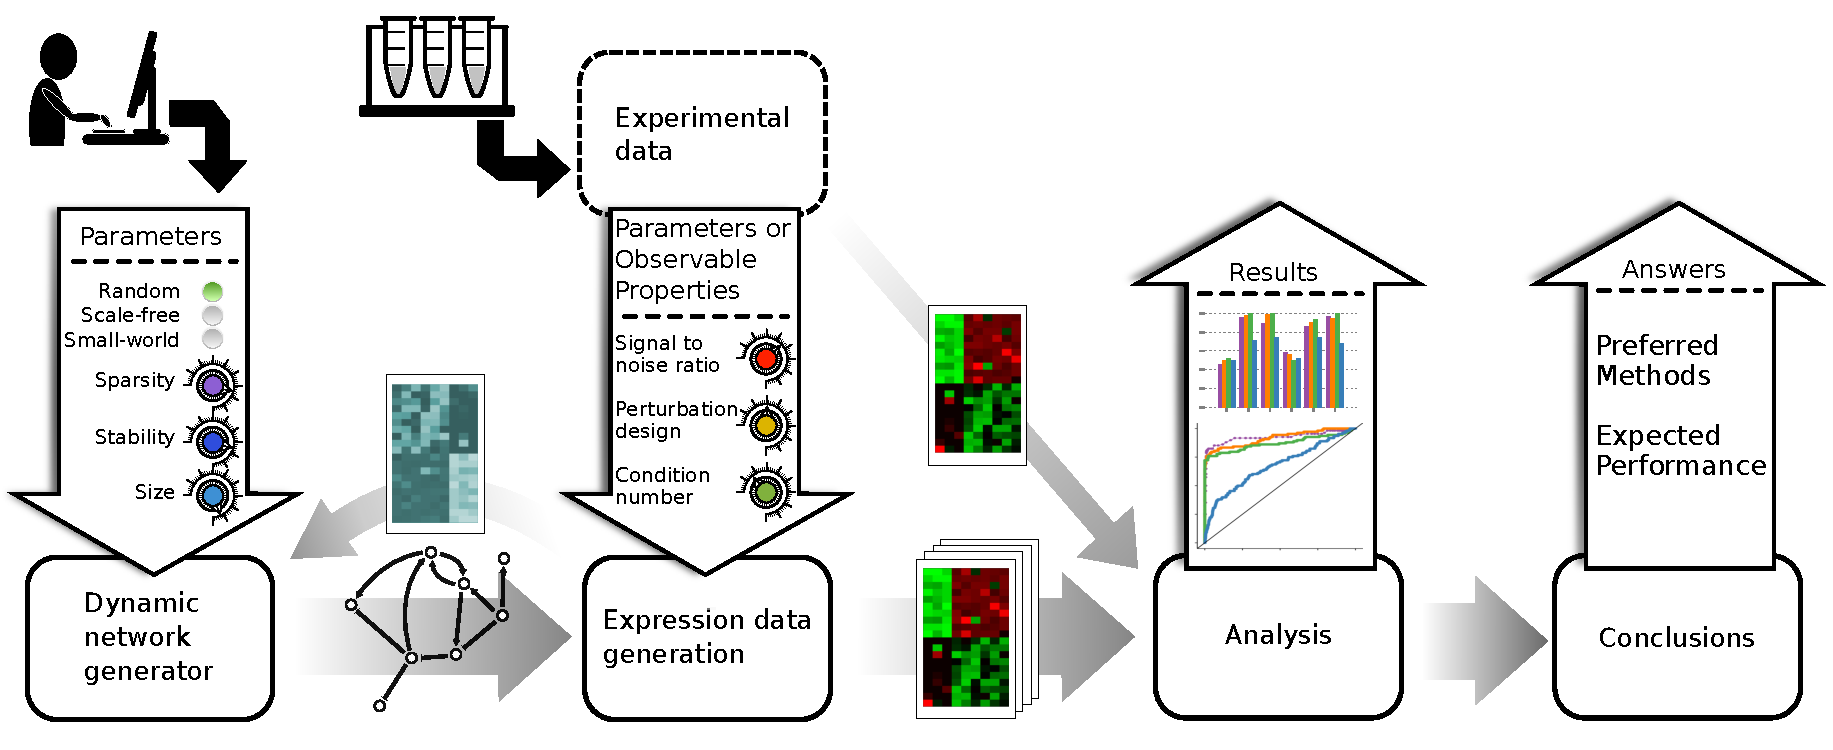
\includegraphics[width=0.9\textwidth]{img/pipeline.pdf}
\captionsetup{width=0.9\textwidth}
\caption{Schematic workflow of network and data generation followed by analysis in \gs. (i) Import or generate networks with a range of properties; stabilize and modify the interampatteness degree. (ii) Generate expression data with specific SNR, perturbation design, and condition number. (iii) Analyze GRN inference benchmark results in relation to the network and data properties. (iv) Draw conclusions about which methods to use under what conditions. The figure also shows an alternative path where \gs extracts properties from experimental data in order to generate simulated networks and data.  Such a benchmark provides information about the expected accuracy for a given real dataset.}
\label{fig:benchmark-pipeline}
\end{figure*}

The network construction process usually involves modelling networks as a system of ordinary differential equations (ODEs), with e.g. linear \citep{Bansal2007}, or nonlinear \citep{VandenBulcke2006,Schaffter2011} models.
The perturbation, \ie system input, used in the experimental design is typically a single gene knockdown/knockout, or a system wide perturbation, \ie a perturbation that randomly alters multiple genes at a time.

To streamline the creation of new benchmarks of network inference methods several packages have been published to facilitate the creation a benchmark data sets and networks \citep{VandenBulcke2006,Hache2009b,DiCamillo2009,Schaffter2011}.
A common feature of these benchmarking packages is the focus on network structure as the main feature controllable by the user.
\emph{\syntren} \citep{VandenBulcke2006} utilizes selected dynamic structures and sub-networks from biological systems, \coli and \yeast.
\emph{\netsim} \citep{DiCamillo2009} takes a different approach by generating dynamical models, incorporating structurally random network motifs, which they dub modular topology models.
\emph{\genge} \citep{Hache2009b} uses a nonlinear model similar to \syntren and allows for the generation of networks with specific network motifs.
All the above methods utilize some form of non-linear dynamics to produce gene expressions from the network structure. 

The GRN inference community has organized around challenges, such as the DREAM
challenge, to benchmark network inference methods by applying them to the same data and comparing their performance \citep{Marbach2012}.
The package \emph{\gnw} \citep{Schaffter2011} expands upon ideas similar to those of the \emph{\syntren} and \emph{\genge} packages and is used to create datasets for these challenges.
\emph{\gnw} enables the user to choose among a variety of \insilico standard perturbation designs when generating networks and time-series data, as well as to define the number of nodes and in-degree.
Its nonlinear dynamical model and simulated data are based on several types of omics data in order to mimic a real biological system.

Publicly available gene expression datasets typically suffer from few data points compared to the high number of genes and possible interactions, large measurement uncertainty both in the perturbations and responses, \ie poor signal to noise ratio (SNR), and redundant nearly collinear variables, \ie ill-conditioned data matrices \citep{Nordling2013phdthesis}.
Considering this, previously published benchmark packages support surprisingly few perturbation design alternatives and data properties.
Noise is typically added to the input and/or output as a percentage of the magnitude of the applied perturbation or measured signal, rather than the SNR. Due to the ill-conditioning, the former does not typically allow for control of the later.
% \textcolor{red}{
In a similar ambition as Kurtz et al.\cite{SPIEC-EASI2015}, we seek to control certain aspects of data generation.%}
However, no previously published package makes it clear to what extent the specific model, or the perturbation design, effects the data generated or the inference being made.
None of the previously published packages facilitate this analysis. Nor do they facilitate control of observable data properties, such as the SNR and ill-conditioning, which as we have demonstrated should be used to guide the algorithm selection \citep{Tjarnberg2014}.

The DREAM challenge, for example, does not define observable properties that could guide a choice of inference method or give an estimate of how informative the dataset is. Instead it focuses on network properties and motifs when trying to evaluate to what extent a specific inference approach is useful.
While this might reveal hard to infer motifs and network structures, it becomes meaningless when faced with a dataset since the motifs can not be observed a priori.
Furthermore, the perturbation design is not connected to the network properties, thus equal perturbation design could give arbitrarily "good" or "bad" data given a specific network model.
While an algorithm may generally perform well, it might act to the contrary faced with a specific set of data properties.

% \textcolor{red}{
A more recent benchmarking package, \netbenchmark \citep{Bellot2015}, aims to evaluate inference methods by bundling datasets from \emph{Rogers simulator}\cite{rogers2005bayesian}, \emph{\syntren}  and \emph{\gnw}, and benchmarking across several existing inference algorithms in a unified workbench. However, the fundamental issues of the methods aggregated are neither solved nor addressed, simply evaluated in the same way.%}
Benchmarks should provide guidance on both (i) which inference method to use for a particular dataset, and (ii) which errors to expect in the inferred network. Benchmarking should be a data driven procedure.

Here we present \gs, a benchmarking suite designed specifically to deal with the issues presented above.
\gs focuses on key properties influencing inference performance \cite{Tjarnberg2014}, allowing the user to "tune" certain parameters in the context of the core functionality expected from a benchmarking suite. 
In the generation of the dynamical network model, \gs focuses on stability\cite{Zavlanos2011} and interampatteness \cite{Nordling2009}.
By interampatteness we mean the ratio between the system's ability to amplify and attenuate different signals, which for a linear system corresponds to the condition number of the network matrix. This is strongly correlated with the difficulty of inferring the correct network, as attenuated signals typically are hidden in the noise and essentially determines the accuracy of the inferred network, since network inference is an inverse problem\cite{Nordling2013phdthesis}.

The observed signal is determined by the applied perturbation and the attenuation of it by the system. The strength of the perturbations could and should be scaled to counteract the intrinsic attenuation of signals.
The condition number of the dataset has been shown to serve as a proxy for the interampatteness in the context of known perturbations\cite{Nordling2013phdthesis,Tjarnberg2014}. 
The benefit here is that the condition number of the dataset can be observed and hence provide information on how difficult it is to infer a specific network from the available data.

The noise estimate in the direction of the data's smallest variation is expected to have the greatest impact on the data quality, as in any inverse problem.
Therefore we provide variation estimates and apply noise scaled towards the principle directions of variance in the data (by default the smallest).
Since the variation in the data can be distributed very differently among the directions from one dataset to the next, this is necessary to correctly see what effect a certain level of noise can have on the data.
This makes it possible to have two observable properties, signal to noise ratio and the condition number of the data, as tune-able parameters not previously incorporated into benchmarking pipelines, yet informative for property-dependent error analysis and confidence estimation. 
This informs the user how informative the data set is and what performance should be expected from different methods, as shown previously \cite{Tjarnberg2013,Tjarnberg2014}.

\gs improves upon existing packages by providing a data driven approach to benchmarking focused on independently controlling properties of network and data. This is essential for establishing the relation between properties and inference accuracy. One of the most important questions in network inference is what accuracy can be expected for a given real dataset. \gs is able to address this question by extracting salient properties from experimental data and then generate simulated networks and data that closely match these properties (See Figure \ref{fig:benchmark-pipeline}).
In this article we demonstrate the workflow of \gs Figure \ref{fig:benchmark-pipeline}, with code examples given in the Supplementary Information, in order to lower the initial usage threshold, focusing on generating approximations with tuned properties and avoiding unnecessary complexity in order to gain insight.

